%!TEX root = main.tex

\section{How do software developers \textbf{evaluate} merge conflict resolutions? (RQ3)}\label{RQ3}

After implementing a merge conflict resolution, software developers must evaluate whether their resolution has returned the codebase to a clean state.
We asked developers to select the conditions (from interviews) that they use to determine whether their resolution has successfully addressed the merge conflict.

\subsection{Success Conditions for Merge Conflict Resolutions}

In the \textit{Exploratory Interviews}, developers described six common conditions they considered important in their evaluation.
We asked \textit{Processes Survey} participants to select from this list of conditions, including an \textit{Other} option to elicit additional conditions.
Only two developers selected that condition, indicating ``performance tests showing similar performance'' and ``client approval.''
We received 324 selections from 89 participants and present the aggregated results in Table~\ref{conditionsSuccess}.

\begin{table}[!htbp]
\caption{Conditions of Successful Merge Conflict Resolutions from \textit{Processes Survey}\textsuperscript{i}}
\label{conditionsSuccess}
\centering
\begin{tabularx}{\textwidth}{lr|*{7}{C}c@{}}
\toprule
  \rowcolor[gray]{0.85}
  & & C1 & C2 & C3 & C4 & C5 & C6 & C7 \\
\midrule
	C1 & All tests pass & \textbf{67} & & & & & & \\
	\rowcolor[gray]{0.95}C2 & Code compiles & 50 & \textbf{67} & & & & & \\
	C3 & Code looks correct & 50 & 54 & \textbf{66} & & & & \\
	\rowcolor[gray]{0.95}C4 & VCS warmings gone & 38 & 42 & 41 & 51 & & & \\
	C5 & Code reviewed & 32 & 31 & 27 & 25 & 38 & & \\
	\rowcolor[gray]{0.95}C6 & Merged to production & 27 & 27 & 27 & 26 & 19 & 33 & \\
	C7 & Other & 2 & 2 & 0 & 0 & 0 & 0 & 2 \\
\bottomrule
    \multicolumn{9}{c}{\noindent\parbox[t]{11.7cm}{\vspace{0.4em}\textsuperscript{i}\hspace{0.2em}\textit{Processes Survey} participants were allowed to select multiple conditions. Each entry represents the number of participants that selected both of the conditions indicated for the column and row. 68 out of 102 participants (67\%) selected three or more conditions.}\vspace*{-0.3\baselineskip}} \\
\end{tabularx}
\end{table}

\textit{All tests pass} (C1), \textit{code successfully compiles} (C2), and \textit{code looks correct (i.e. visual test passes)} (C3) were the most commonly selected conditions required for a successful merge resolution.
These results are in line with existing literature showing that testing (C1) can be used for validating program functionality and correctness~\cite{beizer1984software,tian2005software}. %and have been fundamental to development processes such as test-driven development for several years~\cite{beck2003test}.
Similarly, the use of compilers to validate code (C2) as being executable and in good-working order will be familiar to any developer using a compiled programming language.

The use of visual inspection as a measure of successful merge conflict resolutions is surprising to us, given that \textit{complexity of conflicting lines of code}~(F1) is the highest rated factor for impact on merge conflict difficulty~\cite{mckee2017software}.
Inspecting code requires time and expertise in the area of conflicting code.
However, the survey participants that selected \textit{code looks correct (i.e. visual test passes)}~(C3) had a mean of 9.2 years of programming experience, which is only slightly higher than the overall mean of 9.1 years of programming experience.

Looking at the combination of \textit{code looks correct (i.e. visual test passes)}~(C3) with the other conditions, we find that 54 participants also selected \textit{all tests pass}~(C1) (52.9\%).
As the most common co-occuring selections, we conclude that although developers rely upon their expertise to visually inspect a merge conflict resolution, they also run the test suite to validate their evaluation.
Experience can play a big factor, as this visual method (C3) is highly subjective.

\boldif{Tests are still the most common criteria for determining a merge conflict resolution successful.}
The two most common evaluation criteria that developers mentioned are that the \emph{code compiles,} and that \emph{all tests pass.}
However, less then half selected both options.
While tests passing can be considered a good criteria of a successful resolution, the fact that the code compiles is not.
Even if the code compiles, there can be logical errors that are introduced during the merge resolution process, especially if the resolution was difficult.

\boldif{Only a minority of developers mention that code review is part of their success criteria}
Interestingly, only a minority of developers (37.25\%) mentioned code reviews as part of their success criteria.
%TODO add citation for the code review part
While code reviews are an effective way to detect bugs introduced by changes in the codebase, the practice appears to have not been adopted for code changed during merge conflict resolutions.

\subsection{Merge Resolution Evaluation Toolsets}

From the \textit{Exploratory Interviews}, we identified five categories of software development tools that developers mention in relation to merge conflicts.
In the \textit{Processes Survey}, we asked the developers to identify the tools they use when evaluating a merge conflict resolution.
We received 204 selections from 89 participants.
The aggregated results are presented in Table~\ref{resolution-evaluation-tools}, ranked according to the percentage of participants that selected each toolset.

\begin{table}[!htbp]
\renewcommand{\arraystretch}{1.2}
\caption{Merge Resolution Evaluation Toolsets from \textit{Processes Survey}}
\label{resolution-evaluation-tools}
\centering
\begin{tabularx}{\textwidth}{Q{10.05cm}|cr}
\toprule
  \rowcolor[gray]{0.85}
  \parnoteclear % tabularx will otherwise add each note thrice
  Description & Selections\parnote{\label{toolsets}\textit{Processes Survey} participants were allowed to select multiple toolsets. 64 out of 89 participants (71.91\%) selected multiple toolsets.} & Percentage\parnoteref{toolsets} \\
\midrule
  Version Control Systems (e.g. Git, Subversion, CVS) & 82 & (92.14\%) \\
  \rowcolor[gray]{0.95}Continuous Integration (e.g. TravisCI, Jenkins, TFS) & 62 & (69.66\%) \\
  Program Analysis Tools (e.g. Coverity, CodeSonar) & 26 & (29.21\%) \\
  \rowcolor[gray]{0.95}DevOps Tools (e.g. Nagios, Monit, Kabana) & 17 & (19.10\%) \\
  Release Management Tools (e.g. Chef, Puppet, Salt) & 9 & (10.11\%) \\
  \rowcolor[gray]{0.95}Other Tools & 8 & (8.99\%) \\
\bottomrule
\end{tabularx}
\parnotes
\end{table}

By far, the most selected tools were \textit{version control systems} (VCS) and \textit{continuous integration} (CI) platforms, with 82 (92.14\%) and 62 (69.66\%), respectively.
The mean for all other tool categories was 15 selections (16.85\%), and represents a combined 29.4\% of response selections.

The use of version control systems to determine whether a resolution was successful aligns with the \textit{VCS warnings are gone} (C3) condition.
Also, continuous integration is dependent on code being compilable (C2), and tests being written and maintained (C1).
However, the availability of tools for evaluating merge conflict resolutions might constrain the conditions that developers are willing to consider for their merge conflict resolutions to be successful.
Further research is needed to determine whether there is a causal relationship between these dimensions, and whether more effective conditions could be supported by merge conflict toolsets.

\boldif{Some approaches will only detect direct merge conflicts, not indirect ones.}
Not all of the tools developers use for evaluating the result of a merge conflict resolution can detect all types of merge conflicts.
For example, Version Control Systems will detect only direct conflicts.
Even if the conflict is solved, from the version control systems' perspective, there still might be build or test issues.
Indirect conflicts might slip through if the developer does not run the test suite after resolving the conflict.
While almost 70\% of our participants mentioned that they used Continuous Integration as part of the evaluation process, those that don't might be inadvertently introducing bugs when they resolve the merge conflict.

\boldif{There is a lack of tool support that makes it difficult for developers to properly evaluate the success of a merge conflict resolution.}
Finally, developers have to manually check if their merge resolution is correct.
This is done, either by checking that the version control warnings are gone, inspecting the code for any mistakes, or by manually running the tests.
We notice that there is a lack of an automated process.
Without it the developer might, willingly or unwillingly, skip steps.
Also, this lack of a comprehensive toolset might hamper new developers in their efforts to successfully resolve merge conflicts.

\subsection{Backup Strategies}

Merge conflict resolutions are not always successful.
When they fail, developers must alter their patch and potentially switch strategies in order to successfully resolve the conflict.

To understand the prevalence of failed conflict resolutions, we asked \textit{Processes Survey} participants to indicate the frequency in which their first attempt at resolving a merge conflict fails (see Table~\ref{first-attempt-failure}).
The most common response was \textit{somewhat infrequently} (mean: $3.49$ on a 5-point Likert-type scale).
This suggests that first attempts typically succeed.
However, this also shows that 78.7\% of participants (70 out of 89) occasionally fail at their first attempt and must make additional attempts to resolve a merge conflict.
We also observe that the frequency of failed first attempts follows software development experience; where the least experienced developers experience failed first attempts most often.

\begin{table}[!htbp]
\renewcommand{\arraystretch}{1.2}
\caption{Frequency of Failure on First Attempts at Merge Conflict Resolution from \textit{Processes Survey}}
\label{first-attempt-failure}
\centering
\begin{tabularx}{\textwidth}{lQ{5.1cm}|A{1.6cm}Q{1.9cm}|A{2.7cm}}
\toprule
  \rowcolor[gray]{0.85}
  \parnoteclear % tabularx will otherwise add each note thrice
  & Frequency & Selections\parnote{89 out of 102 participants (87.26\%) indicated a frequency.} & Percentage & Dev. Experience\parnote{Mean software development experience for participants that indicated a specific frequency.} \\
\midrule
  1 & Very frequently & 4 & (4.49\%) & 6.00 years \\
  \rowcolor[gray]{0.95}2 & Somewhat frequently & 13 & (14.61\%) & 7.31 years \\
  3 & Occasionally & 26 & (29.21\%) & 9.27 years \\
  \rowcolor[gray]{0.95}4 & Somewhat infrequently & 27 & (30.34\%) & 10.15 years \\
  5 & Very infrequently & 19 & (21.35\%) & 9.42 years \\
\bottomrule
\end{tabularx}
\parnotes
\end{table}

%\begin{figure}
%	\centering
%	\fbox{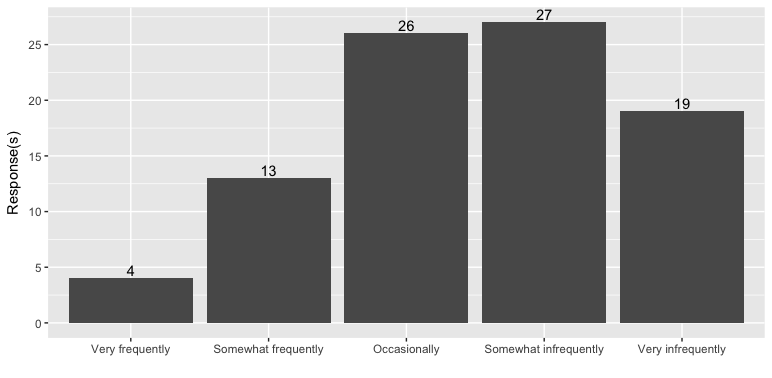
\includegraphics[width=0.95\textwidth,keepaspectratio]{FirstAttemptFailure}}
%	\caption{Frequency of Failures in First Attempts at Merge Conflict Resolution. Scale: 1 is \textit{Very frequently} and 5 is \textit{very infrequently}. 89 out of 102 participants (87.26\%) indicated a frequency in the \textit{Processes Survey}.\vspace*{-0.3\baselineskip}}
%	\label{fig:first-attempt-failure}
%\end{figure}

Furthermore, we asked survey participants to describe their backup strategies when their first attempt at resolving a merge conflict fails.
We received 75 responses and the aggregate results are presented in Table~\ref{backup-strategies}, ranked according to the percentage of participants that described using each backup strategy.

Developers' backup strategies include \textit{take it offline} (B1), \textit{collaborating} (B2), \textit{try again} (B3), \textit{redoing changes} (B4), and \textit{no backup strategy} (B5).
Since \textit{no backup strategy} (B5) is not a strategy in and of itself, we focus on strategies B1--B4 instead.

The \textit{take it offline} (B1) strategy involves moving conflicting code away from shared branches or code repositories, and working locally to resolve the conflict without disrupting other developers.
The antithesis of this strategy is \textit{collaborating} (B2), where developers seek out other developers that are more knowledgeable about the area of conflicting code.
The B1 and B2 strategies contrast each other, and show that developers reserve more costly strategies (in terms of time, effort, and coordination) as backups to their primary resolution strategies.
The most common backup strategies, are in a way, opposite of the primary strategies.

\begin{table}[!htbp]
\renewcommand{\arraystretch}{1.2}
\caption{Backup Strategies for Resolving Merge Conflicts from \textit{Processes Survey}}
\label{backup-strategies}
\centering
\begin{tabularx}{\textwidth}{c|Q{7.75cm}|cr}
\toprule
  \rowcolor[gray]{0.85}
  \parnoteclear % tabularx will otherwise add each note thrice
  Strategy & Description & Participants\parnote{\label{backups}75 out of 102 participants (73.53\%) provided a description of their backup strategy.} & Percentage\parnoteref{backups} \\
\midrule
  B1 & Take it offline & 19 & (25.33\%) \\
  \rowcolor[gray]{0.95}B2 & Collaborating & 17 & (22.67\%) \\
  B3 & Try again & 15 & (20.00\%) \\
  \rowcolor[gray]{0.95}B4 & Redoing changes & 14 & (18.67\%) \\
  B5 & No backup strategy\hspace{2.0cm} & 10 & (13.33\%) \\
\bottomrule
\end{tabularx}
\parnotes
\end{table}
\vspace{0.8em}

Additionally, we find that developers also simply \textit{try again} (B3) to merge the same code together and hope that their tools are able to succeed with a second attempt.
Developers also resort to \textit{redoing changes} (B4), by way of reverting and manually recreating the changes found in conflicting commits when their initial attempt failed.
The B3 and B4 strategies appear to cement the extremes of the cost spectrum of backup strategies for resolving merge conflicts.
Simply retrying the same merge (B3) requires very little additional work.
It implies that developers think that they might have missed something, and that by going through the changes again, they might catch or have a better understanding of the two changes that are conflicting.
However, the process of redoing changes (B4) is a duplication of previous efforts. %and is therefore costly on developer's time.
This \textit{Nuclear Option} is clearly a time-consuming strategy for developers (both in planning and implementing a resolution), and yet the perceived costs of trying to unravel the conflicting code appear to be higher than the costs of reimplementing features.

\boldif{Some developers do not have an approach for dealing with merge conflicts.}
Finally, an interesting result is that some developers do not have a strategy for approaching a merge conflict resolution.
The existence of this \textit{no strategy} approach is anecdotal, but curious, since we assume that developers are rational actors seeking to organize themselves in ways that increase the likelihood of successful outcomes.
Yet this strategy appears to go counter to that notion.
One explanation for the lack of a strategy is the lack of experience.
With a mean of 3.5 years of programming experience (5.6 years less than the overall mean), these participants might not have encountered enough situations to form a coherent strategy.

Interestingly, when developers perceive a merge conflict to be too difficult to resolve they occasionally resort to removing all conflicting code and reimplementing the underlying functionality in order to fix it.